% \documentclass[tikz]{standalone}
% 
% \usepackage{ucs}
% \usepackage[utf8]{inputenc}
% \usepackage{fontenc}
% \usepackage{graphicx}
% 
% \usepackage[]{hyperref}
% 
% 
% \usepackage{verbatim}
% \usetikzlibrary{positioning} %
% 
% \author{Jose Teixeira}
% \date{06/14/18}
% 
% \begin{document}


\newlength\yearposx
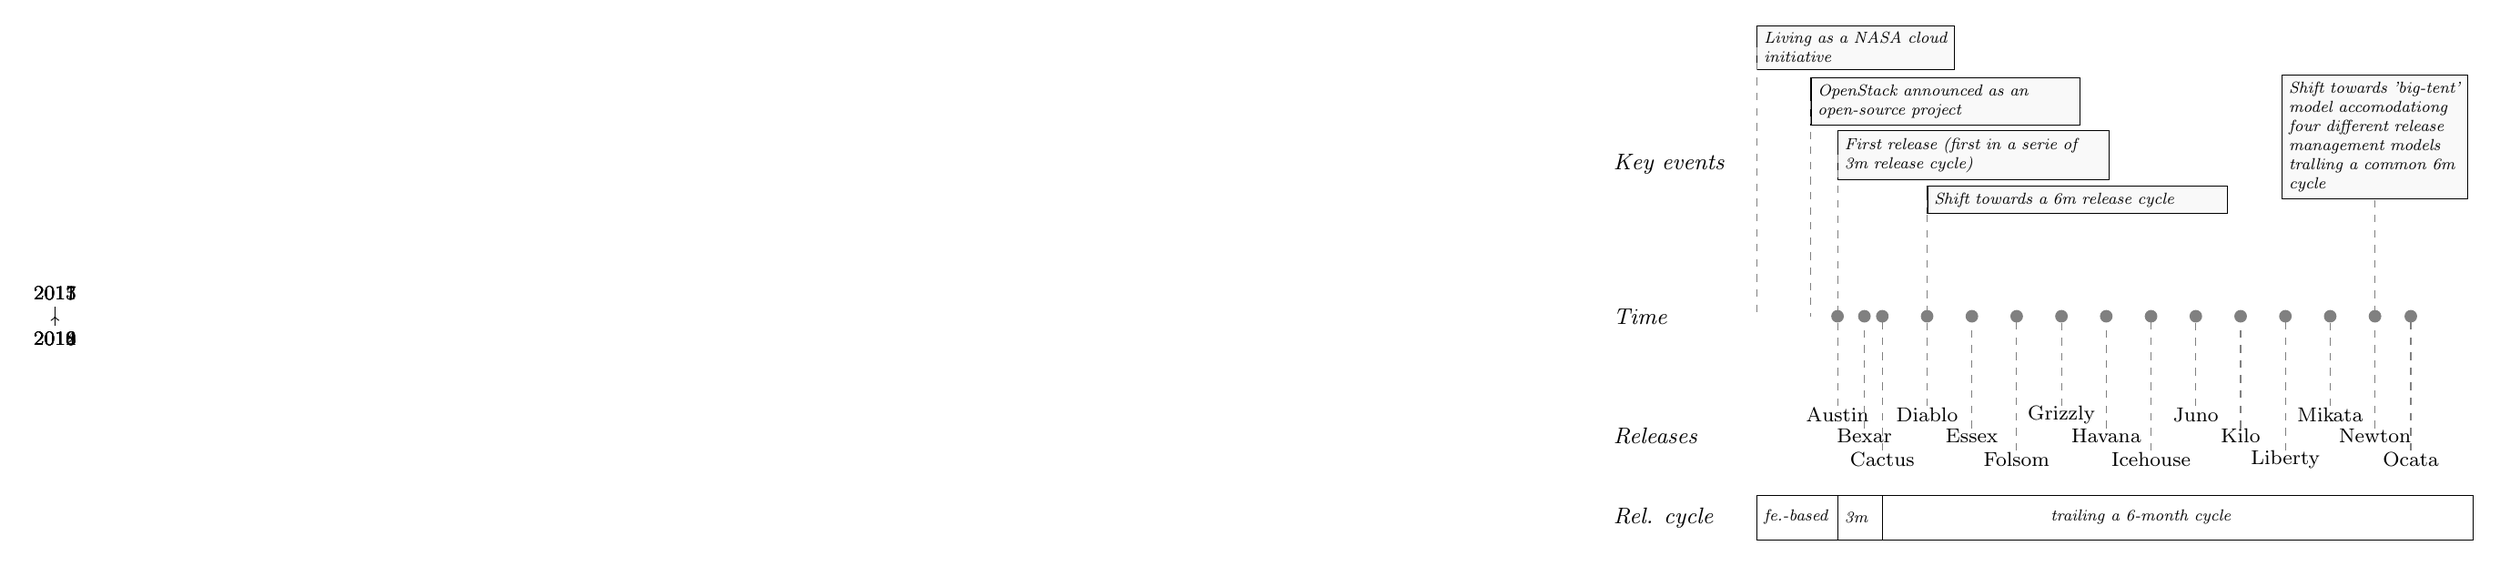
\begin{tikzpicture}[scale=1.25]
   

    % define coordinates (begin, used, end, arrow)
    \foreach \x in {2010,2011,2012,2013,2014,2015,2016,2017,2018}{
        \pgfmathsetlength\yearposx{(\x-1990)*1cm};
        \coordinate (y\x)   at (\yearposx,0);
        \coordinate (y\x t) at (\yearposx,+3pt);
        \coordinate (y\x b) at (\yearposx,-3pt);
    }
    

% rectangle 
%\shade [left color=black,right color=white]  (2010-1990,04) rectangle (2013-1990,-1);
    


\begin{scope}[every node/.style={font=\small\itshape}]

% % Draw key events legend  

\node at (2010-1990-1.7,1.7) [right] {\small Key events};

  
  
% % Draw time legend 

\node at (2010-1990-1.7,0) [right] {\small Time};

% % Draw releases legend  

\node at (2010-1990-1.7,-1.33) [right] {\small Releases};



% % Draw key release cyle  

\node at (2010-1990-1.7,-2.25) [right] {\small Rel. cycle};

\end{scope}


% Key event 1

  \node[scale=0.8, draw, align=left,fill=white!95!gray,text width=3.2cm, font=\itshape\footnotesize, right] at (2010-1990,3) 
  (EV1)   {Living as a NASA cloud initiative};

  \path[dashed] (2010-1990,3) edge [gray] (2010-1990,0);

% Key event 2

  \node[scale=0.8,draw, align=left,fill=white!95!gray,text width=4.45cm, font=\itshape\footnotesize, right] at (2010.6-1990,2.4) 
  (EV1)   {OpenStack announced as an open-source project}; 
  
  \path[dashed] (2010.6-1990,2.4) edge [gray] (2010.6-1990,0);
    
    
% Key event 3

  \node[scale=0.8,draw, align=left,fill=white!95!gray,text width=4.5cm, font=\itshape\footnotesize, right] at (2010.9-1990,1.8) 
  (EV1)   {First release (first in a serie of 3m release cycle)}; 
  
  \path[dashed] (2010.9-1990,1.8) edge [gray] (2010.9-1990,0);    

 
    
% Key event 4

  \node[scale=0.8,draw, align=left,fill=white!95!gray,text width=5cm, font=\itshape\footnotesize, right] at (2011.9-1990,1.3) 
  (EV1)   {Shift towards a 6m release cycle}; 
  
  \path[dashed] (2011.9-1990,1.3) edge [gray] (2011.9-1990,0);    

 
 
 % Key event 5

  \node[scale=0.8,draw, align=left,fill=white!95!gray,text width=3cm, font=\itshape\footnotesize] at (2016.9-1990,2) 
  (EV1)   {Shift towards 'big-tent' model accomodationg four different release management models tralling a common 6m cycle}; 
  
  \path[dashed] (2016.9-1990,1.3) edge [gray] (2016.9-1990,0);    

  
  
  
  
    % draw horizontal line with arrow
    \draw [->] (y2010) -- (y2018);
    % draw ticks
   \foreach \x in {2010,2011,2012,2013,2014,2015,2016,2017,2018}
        \draw (y\x t) -- (y\x b);
 
 % annotate
    \foreach \x in {2010,2012,2014,2016,2018}
        \node at (y\x) [below=3pt] { {\footnotesize \x}};
    \foreach \x in {2011,2013,2015,2017}
        \node at (y\x) [above=3pt] {{\footnotesize \x}};
       
       
     \node at (2010.9-1990,-1.1) (A)  {\footnotesize Austin};
     \node at (2011.2-1990, -1.33) (B)  {\footnotesize  Bexar};
     \node at (2011.4-1990,-1.6) (C)  {\footnotesize  Cactus};
     \node at (2011.9-1990,-1.1) (D)  {\footnotesize  Diablo};
     \node at (2012.4-1990,-1.33) (E) {\footnotesize  Essex};
     \node at (2012.9-1990,-1.6) (F)  {\footnotesize Folsom};
     \node at (2013.4-1990,-1.1) (G)  {\footnotesize Grizzly};
     \node at (2013.9-1990,-1.33) (H)  {\footnotesize Havana};
     \node at (2014.4-1990,-1.6) (I)  {\footnotesize Icehouse};
     \node at (2014.9-1990,-1.1) (J)  {\footnotesize Juno};
     \node at (2015.4-1990,-1.33) (K) {\footnotesize Kilo};
     \node at (2015.9-1990,-1.6) (L)  {\footnotesize Liberty};
     \node at (2016.4-1990,-1.1) (M)  {\footnotesize Mikata};
     \node at (2016.9-1990,-1.33) (N)  {\footnotesize Newton};
     \node at (2017.3-1990,-1.6) (O)  {\footnotesize Ocata};
%      \node at (2017.8-1990,-2.5) (P) [gray,left] {\footnotesize Pike};
%      \node at (2017.8-1990,-2) (Q) [gray,left] {\footnotesize Queens};
% 


      
     % A 
     \fill [gray] (2010.9-1990,0) circle (2pt);
     \path[dashed] (2010.9-1990,-1) edge [gray]  (2010.9-1990,0);s
      
     %B 
     \fill [gray] (2011.2-1990,0) circle (2pt);
     \path[dashed] (2011.2-1990,-1.25) edge [gray] (2011.2-1990,0);
     
     %C 
     \fill [gray] (2011.4-1990,0) circle (2pt);
     \path[dashed] (2011.4-1990,-1.5) edge [gray] (2011.4-1990,0);
     
     %D
     \fill [gray] (2011.9-1990,0) circle (2pt);
     \path[dashed] (2011.9-1990,-1.0) edge [gray] (2011.9-1990,0);
     
     %E 
     \fill [gray] (2012.4-1990,0) circle (2pt);
     \path[dashed] (2012.4-1990,-1.25) edge [gray] (2012.4-1990,0);
     
     
     % F 
     \fill [gray] (2012.9-1990,0) circle (2pt);
     \path[dashed] (2012.9-1990,-1.5) edge [gray] (2012.9-1990,0);
     
     
     % G 
     \fill [gray] (2013.4-1990,0) circle (2pt);
     \path[dashed] (2013.4-1990,-1.0) edge [gray] (2013.4-1990,0);
     
     % H
     \fill [gray] (2013.9-1990,0) circle (2pt);
     \path[dashed] (2013.9-1990,-1.25) edge [gray] (2013.9-1990,0);
     
     % I 
     \fill [gray] (2014.4-1990,0) circle (2pt);
     \path[dashed] (2014.4-1990,-1.5) edge [gray] (2014.4-1990,0);
     
       
     % J 
     \fill [gray] (2014.9-1990,0) circle (2pt);
     \path[dashed] (2014.9-1990,-1.0) edge [gray] (2014.9-1990,0);
       
     % K 
     \fill [gray] (2015.4-1990,0) circle (2pt);
     \path[dashed] (2015.4-1990,-1.25) edge [gray] (2015.4-1990,0);
     
     
     % L
     \fill [gray] (2015.9-1990,0) circle (2pt);
     \path[dashed] (2015.9-1990,-1.5) edge [gray] (2015.9-1990,0);
     
     
     
     % M 
     \fill [gray] (2016.4-1990,0) circle (2pt);
     \path[dashed] (2016.4-1990,-1) edge [gray] (2016.4-1990,0);
     
     
     % N 
     \fill [gray] (2016.9-1990,0) circle (2pt);
     \path[dashed] (2016.9-1990,-1.25) edge [gray] (2016.9-1990,0);
     
     
     
     % O 
     \fill [gray] (2017.3-1990,0) circle (2pt);
     \path[dashed] (2017.3-1990,-1.5) edge [gray] (2017.3-1990,0);
     

%       \node[draw, align=center,fill=yellow!80!black,text width=5cm,text height=8pt] at (2011-1990,2) (E1)   {OpenStack starts as a \\ open-source project outside NASA};
% %     

% release cycle 



%\shade [fill=gray!120!black,draw opacity=0.5] (2010-1990,04) rectangle (2013-1990,-1);
%\node at (2010-1990-0.28,-2.5) [anchor=center, above=2pt+2pt,draw, font=\itshape\footnotesize,right, text height=3pt] {f. based};
\draw (2010-1990,-2) rectangle (2010.9-1990,-2.5) ;
\node at (2010-1990,-2.27) [scale=0.8,font=\itshape\footnotesize,, right, text height=3pt] {fe.-based};



%\shade [fill=gray!130!black,draw opacity=0.5] (2013-1990,04) rectangle (2015-1990,-1);
%\node at (2010.9-0.08-1990,-2.5) [anchor=center, above=2pt+2pt,draw, font=\itshape\footnotesize, right, text height=3pt] {3 m.};
\draw (2010.9-1990,-2) rectangle (2011.4-1990,-2.5);
\node at (2010.9-1990,-2.27) [scale=0.8,font=\itshape\footnotesize,, right, text height=3pt] {3m};


%\shade [] (2015-1990,04) rectangle (2018-1990,-1);
%\node at (2016.5-1990,-2.5) [anchor=center,  above=2pt+2pt,draw, font=\itshape\footnotesize, right, text height=3pt] { 6 m.};

\draw (2011.4-1990,-2) rectangle (2018.0-1990,-2.5);
\node at (2013.2-1990,-2.27) [scale=0.8,font=\itshape\footnotesize, right, text height=3pt] {trailing a 6-month cycle};

% %     

\end{tikzpicture}
 
 
%\end{document}
